\documentclass[a4paper,11pt,singlespacing]{article}

\usepackage{setspace}
\usepackage[utf8]{inputenc}
\usepackage[T1]{fontenc}
\usepackage{graphicx}
\usepackage{color}
\usepackage{hyperref}
\usepackage{listings,xcolor}

\renewcommand{\figurename}{Abbildung}

\graphicspath{ {./images/} }



\begin{document}
	\setlength{\parindent}{0ex}
	\begin{titlepage}

        \author{Luca Asmus\\ Marius Würstle\\Rolf Wiersch}
        \title{Projektskizze: WLAN-AP mit regelmäßigem PSK-Tausch und QR-Code Anmeldung \vspace{10cm}}
        \date{\today}
	    \maketitle
        \thispagestyle{empty}
    \end{titlepage}
	
	\section{Motivation}
	Der Hauptgrund für dieses Projekt war es die Sicherheit im eigenen Gast-WLAN zu gewährleisten, unter Berücksichtigung der Faulheit und Bequemlichkeit vieler Endnutzer. \\ \\
	Wenn Gäste in der heimischen Wohnung auftauchen, ist der Wunsch nach freiem WLAN meist sehr groß. Bedeutet, der pre-shared key muss abgelesen und den Gästen bekannt gemacht werden. Folgend muss dieser umständlich von Hand eingegeben werden. Um hierbei Sicherheit zu gewährleisten, ist dieser meist länger und kryptisch gewählt. Dies führt oft zu falschen Eingabe bzw. Mehrversuchen und darauf folgenden Ärger darüber. Weiterhin ist es vom Gastgeber nicht immer erwünscht, dass die Gäste nach der Verabschiedung den Zugriff zum WLAN behalten. \\ \\
	Da die geschilderten Umstände den Verfassern dieses Dokumentes nicht fremd sind, soll mit diesem Projekt eine eigenständige Lösung erstellt werden. Der Fokus liegt auf einfacher Bedienung und komfortabler Sicherheit. Weiterhin wird für die Sicherheit auf fertige Endprodukte von Drittanbietern verzichtet. 
	
	
	\section{Problem}
	Wie im vorherigen Abschnitt erwähnt, ist vielen Endnutzer die eigene Bequemlichkeit sehr wichtig. Daraus resultiert, dass der pre-shared Key eines WLANs in den meisten Netzwerken einmal oder nie geändert wird. Dadurch können Gäste dauerhaften Zugang zum Netzwerk behalten, obwohl das nicht erwünscht ist.  
	Dies hat zur Folge, dass sich sobald einmal das Passwort  bewusst/unbewusst weitergegeben wurde, jeder mit dem Access-Point verbinden kann. Negative Auswirkungen könnten sich äußern in Form von Missbrauch des Internetzuganges oder durch Angriffe auf das interne Netzwerk. \\ \\ 
	Ein weiteres Problem ist die Umständlichkeit einen sicheren pre-shared Key zu verwenden. Es führt zu unangenehmen Mehraufwand eine kryptische und lange Zeichenkette auf Endgeräten einzugeben bzw. zu merken, den viele Endnutzer nicht eingehen wollen. Deshalb werden oft einfache pre-shared Keys in Form von z.B Wortkombinationen verwendet. Dies hat zur Folge, dass der Zugang einfacher geknackt werden kann.
	
	\section{Lösungsansätze}
	Ein Lösungsansatz stellt ein sich automatisch oder auf Tastendruck änderbarer pre-shared Key dar. Der Key wird jeden Montagmorgen um 03:00 Uhr automatisch durch einen "Cron-Job" gewechselt. Ein Taster kann zusätzlich betätigt werden, falls das Passwort sofort geändert werden soll.
	Der Key wird so gewählt, dass er höchstwahrscheinlich nicht in dem Zeitraum geknackt werden kann bis ein neuer erzeugt wird. Durch diese Maßnahme wird die Sicherheit des WLANs verbessert und sichergestellt. \\
	Mit diesem neu generierten Key können sich Endgeräte anmelden und kommunizieren. Hiermit wird das Problem der ungewollten Nutzern gelöst. Diese können sich sobald der Key gewechselt hat, nicht mehr im Netz anmelden. Der Key wird an einem Display in zwei verschiedenen Varianten angezeigt:
	\begin{itemize}
		\item Klartext für Endgeräte ohne Kamera z.B. Laptops
		\item QR-Code zum Scannen für z.B Smartphones
	\end{itemize}

	Es wurde sich für einen QR-Code anstatt eines RFID/NFC Transponder entschieden, da hier die Möglichkeit des Abgreifens des Keys nicht besteht. In Abbildung  \ref{aufbau} ist der Aufbau des Lösungsansatzes graphisch dargestellt. 

	\begin{figure}[ht]
		\centering
		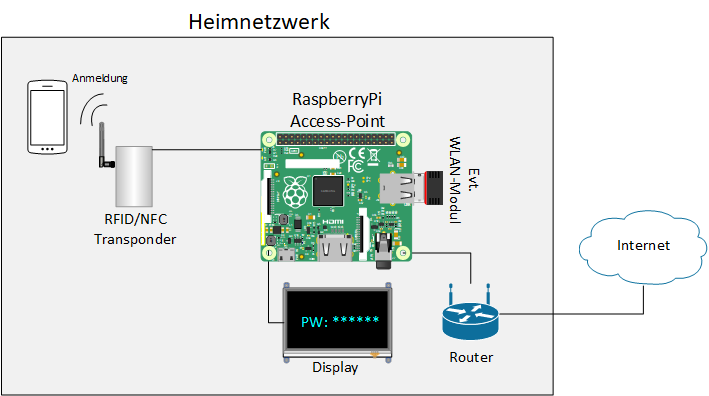
\includegraphics[scale=0.6]{skizze}
			\caption{Aufbau des Gastnetzes}
			\label{aufbau}
	\end{figure}

    Es ist zu erwähnen, dass sich diese Lösung auf die Umsetzung eines Gastnetzes bezieht. Dieses ist getrennt vom restlichen Heimnetz. Es melden sich dort hauptsächlich mobile Geräte an. Dies führt zu einer hohe Fluktuation an Endgeräten im Netzwerk und ist nicht für stationäre Geräte wie z.B Drucker geeignet.
	
	\section{Anforderungsanalyse}

		\subsection{Hardware}
		Für dieses Projekt wird ein Raspberry Pi 3 B+ benötigt. Grund hierfür ist der HDMI Anschlusses, der aus Komfortgründen für das Display benutzt werden soll. Zudem hat dieses Modell ausreichend Leistung, ein integriertes WLAN-Modul und alle nötigen Anschlüsse:
		\begin{itemize}
			\item 2.4GHz and 5GHz IEEE 802.11.b/g/n/ac wireless LAN
			\item Extended 40-pin GPIO header
			\item Full-size HDMI
			\item Micro SD port für das Laden des Betriebsystems und zur Speicherung der Daten
			\item 5V/2.5A DC power input
			\item Ethernet Port
		\end{itemize}
		Zusätzlich wird eine Mikro-SD Karte zum Laden des Betriebsystems und zur Speicherung der Daten benötigt. \\ \\
		Das Display, welches verwendet wird, muss eine ausreichende Auflösung für die Darstellung des QR-Codes besitzen. Deshalb können keine kleineren und billigeren LCD Anzeigen verwendet werden. Außerdem muss dieses noch an den Raspberry Pi in Form von HDMI angeschlossen werden, da die Pins für mögliche Schalter/Umschalter verwendet werden können.
		
		\subsection{Software}
		Um den Raspberry Pi als Access-Point verwenden zu können, müssen zusätzliche Pakete installiert (hostapd) und eine Netzwerkkonfiguration vorgenommen werden. Darunter fällt das Einstellen von DHCP und DNS für die Clients durch "dnsmasq" und Anpassen der IP-Konfiguration. \\ \\
		
		Als Skriptsprache empfiehlt sich Python, da es dort sehr viele Libraries gibt, die einiges an Arbeit abnehmen. Zudem kann man mit Python auf einfache Kommandos des Betriebssystems zugegriffen werden. Für die QR-Code Generierung eignen sich die Libraries "qrcode" und "PyQRCode". 
		
			Als Passwortkonzept wurde sich auf einen 10 Zeichen langen Key geeinigt. Dieser benützt 95 Zeichen in Form von Groß- und Kleinbuchstaben, Zahlen und Sonderzeichen. Begründet wurde diese Entscheidung mit folgender Annahme: \\\\
		Angenommen ein leistungsstarker Rechner schafft durch Brute-Force 2 Billionen Keys pro Sekunde, so würde er 346 Tage benötigen, um alle Keys zu testen.  Wenn schon zur Hälfte der Zeit der richtigen Key gefunden wurde, wäre dies immernoch mehr als ausreichend für eine Woche. Zu sehen ist dies in der folgenden Rechnung:
		\begin{eqnarray}
			(95^{10})\ keys\ \div\ 2000000000000\ \frac{keys}{s} =  29936846.961918945312\ s\\
			29936846.961918945312\ s\ \div\ 60\ \div\ 60\ \div\ 24\ \approx 346 \ Tage\\
			346\ Tage\ \div\ 2\ =\ 173\ Tage
		\end{eqnarray}\\
	    Für die Generierung eines Keys wird das Programm "pwgen" benutzt.
		Zum Schluss müsste der Key durch ein Skript ausgetauscht werden.\\
	
		\subsection{Tests}
		Zu Testzwecken werden unterschiedliche Smartphones (Android/iOS) und Notebooks (Windows/Linux/macOS) benutzt. So soll sichergestellt werden, dass mögliche Probleme aufgrund von Diskrepanzen zwischen den Betriebssystemen bzw. Hardware erkannt werden.
	
	\section{Priorisierung}
	
	Das wichtigste zu Beginn ist, dass die Hardware aufeinander abgestimmt wird. Bedeutet, alle Teile passen zusammen und können angeschlossen werden.
	Danach muss die Konfiguration des Raspberry Pi zum Access-Point erfolgen. Sobald dies funktioniert kann das Generieren des pre-shared Keys und dessen Austausch stattfinden. Folglich wird die Ausgabe des Keys am Bildschirm realisiert. Danach kann dies, um das Generieren des QR-Codes und dessen Ausgabe erweitert werden.\\
	Wenn diese Punkte voll funktional umgesetzt werden konnten, kann sich um einen automatischen oder manuellen Job (bei Tastendruck) zum Generieren und Austauschen des Keys gekümmert werden.
		
		\subsection{Zielgruppe}
		Das Projekt ist für Haushalte geeignet, welche ein sicheres Gästenetz gewährleisten möchten. Es kann außerdem von Firmen genutzt werden, die für Besucher und Mitarbeiter WLAN zur Verfügung stellen möchten und diese nicht für immer in ihrem Netz haben möchten. 
		
		\subsection{Funktionen}
		Im Folgenden werden die verschiedenen Funktionen definiert und kategorisiert.
			\subsubsection{Grundlegende Funktionen}
			\begin{itemize}
				\item Funktionierender Access-Point
				\item DHCP Server
				\item DNS Server
				\item Automatisches Wechseln des Keys
				\item Key Ausgabe als Text
				\item Key Ausgabe als QR-Code
			\end{itemize}
		
			\subsubsection{Optionale Funktionen}
			\begin{itemize}
				\item Anbindung eines Tasters zum manuellen Tausch des Keys 
				\item Energiesparen durch an- und abschalten des Displays
				\item Skript zum Automatisieren der Konfiguration
			\end{itemize}
			
			
			
\end{document}
